\documentclass[13pt,a4paper]{article}
\usepackage[english,german]{babel}
\usepackage[utf8]{inputenc}
\usepackage{color}
\usepackage{hyperref}
\usepackage{mathtools}
\usepackage{amsmath}
\usepackage{graphicx}
\usepackage{tabularx}
\usepackage{amsfonts}

\usepackage{geometry}
\geometry{
  left=3cm,
  right=3cm,
  top=3cm,
  bottom=4cm,
  bindingoffset=5mm
}

\setlength{\parindent}{0em} 
\hypersetup{
    colorlinks=true,
    linktoc=all,
    linkcolor=black,
    urlcolor=black
}

% Hurenkinder und Schusterjungenregel
\clubpenalty = 10000
\widowpenalty = 10000
\displaywidowpenalty = 10000

%Gummi|065|=)
\title{Übung "Statistische Aspekte der Analyse molekularbiologischer und genetischer Daten"}
\author{}
\date{}

% set title of table of contents
\renewcommand*\contentsname{Inhalt}

% https://www.sharelatex.com/learn
% http://www.math.ubc.ca/~cautis/tools/latexmath.html
% http://www.golatex.de/wiki/Kategorie:Befehlsreferenz
% https://en.wikibooks.org/wiki/LaTeX/Mathematics

\begin{document}

\begin{titlepage}

\maketitle
\thispagestyle{empty}
\end{titlepage}
\newpage

\begin{titlepage}
\tableofcontents
\thispagestyle{empty}
\end{titlepage}
\newpage

\section{Übung 1: Biologische Grundlagen – Teil 1}

\subsection{Aufgabe 1}

\begin{itemize}
	\item zu a: siehe Codonsonne\footnote{\url{https://de.wikipedia.org/wiki/Code-Sonne}}\\
		AUG (ATG) als Startcodon, UGA (TGA) als Stopcodon\\
		5' - ATG GTT AAA CAC GTG CAC GAG TGA - 3'\\
		3' - TAC CAA TTT GTG CAC GTG CTC ACT - 5'
	\item zu b:\\
		5' - AUG GUU AAA CAC GUG CAC GAG UGA - 3'
	\item zu c: tRNA für Valin, Lysin, Histidin, Valin, Glutamin, Glutaminsäure (das komplementäre der RNA)
	\item zu d: unpolar/neutral, positiv/basisch, positiv/basisch, unpolar/neutral, polar/neutral, negativ/sauer
	
\end{itemize}

\subsection{Aufgabe 2}

\subsection{Aufgabe 3}

\begin{itemize}
	\item E. coli: $4,6*10^6$ Basen, 4500 Gene
	\item Bäckerhefe: $2*10^7$ Basen, 6000 Gene
	\item Ackerschmalwand: $10^8$ Basen, 25500 Gene
	\item Fruchtfliege (Drosophila Melanogaster): $2*10^8$ Basen, 13500 Gene
	\item Menschen: $3,27 * 10^9$ Basen, 23000 Gene
\end{itemize}

\subsection{Aufgabe 4}

\begin{itemize}
	\item SNP\footnote{\url{https://de.wikipedia.org/wiki/Einzelnukleotid-Polymorphismus}}:
	\begin{itemize}
		\item Single Nucleotide Polymorphism - Einzelnukleotid-Polymorphismus
		\item Variation eines einzelnen Basenpaares in einem DNA-Strang
		\item SNPs sind geerbte und vererbbare genetische Varianten. Begrifflich davon abzugrenzen ist der Begriff der Mutation, der in der Regel eine neu aufgetretene Veränderung bezeichnet
		\item Laktosetoleranz: durch einen SNP im Intron des Gens mcm6 entwickelt, welches 5' von LCT(Lactase) liegt
	\end{itemize}
	\item CNV\footnote{\url{https://de.wikipedia.org/wiki/Gene_copy_number_variants}}:
	\begin{itemize}
		\item Copy number variation - Kopienzahlvariation
		\item struktureller Variation des Erbguts, die Abweichungen der Anzahl der Kopien eines bestimmten DNA-Abschnittes innerhalb eines Genoms erzeugt
	\end{itemize}
	\item Chromosomen-Mutationen\footnote{\url{https://de.wikipedia.org/wiki/Chromosomenmutation}}:
	\begin{itemize}
		\item strukturelle Veränderung eines Chromosoms, 5 Arten
		\item Deletion: Ein Teilstück des Chromosoms (Endstück oder mittlerer Abschnitt) geht verloren
    	\item Translokation: Chromosomen können auseinanderbrechen und dabei Teilstücke verlieren, welche in die Chromatide eines anderen Chromosoms angeheftet werden
	    \item Duplikation: Ein Abschnitt des Chromosoms ist doppelt vorhanden, da ein auseinandergebrochenes Teilstück in die Schwesterchromatide eingegliedert wurde
	    \item Inversion: Innerhalb eines Chromosoms kann sich nach einem doppelten Bruch ein Stück wieder umgekehrt einfügen
	    \item Insertion (auch: Addition): Hier besitzt ein Chromosom ein zusätzliches Teilstück
	\end{itemize}
\end{itemize}

\subsection{Aufgabe 5}
\begin{itemize}
	\item PCR\footnote{\url{https://de.wikipedia.org/wiki/Polymerase-Kettenreaktion}}: Polymerase-Kettenreaktion (polymerase chain reaction)
	\item Prozess besteht aus etwa 20–50 Zyklen, jeder Zyklus besteht aus drei Schritten
	\begin{enumerate}
		\item Denaturierung (Melting, Schmelzen): Zunächst wird die doppelsträngige DNA auf 94–96 $^\circ$C erhitzt, um die Stränge zu trennen. Die Wasserstoffbrückenbindungen, die die beiden DNA-Stränge zusammenhalten, werden aufgebrochen. Im ersten Zyklus wird die DNA oft für längere Zeit erhitzt (Initialisierung), um sicherzustellen, dass sich sowohl die Ausgangs-DNA als auch die Primer vollständig voneinander getrennt haben und nur noch Einzelstränge vorliegen. Manche (sogenannte Hot-Start-) Polymerasen müssen durch eine noch längere anfängliche Erhitzungsphase (bis zu 15 Minuten) aktiviert werden. Danach wird schnell auf 65 $^\circ$C abgekühlt, um die Rückbildung der Doppelhelix zu verhindern.
		\item Primerhybridisierung (primer annealing): Die Temperatur wird ca. 30 Sekunden lang auf einem Wert gehalten, der eine spezifische Anlagerung der Primer an die DNA erlaubt. Die genaue Temperatur wird hierbei durch die Länge und die Sequenz der Primer bestimmt (bzw. der passenden Nukleotide im Primer, wenn durch diesen Mutationen eingeführt werden sollen = site-directed mutagenesis). Wird die Temperatur zu niedrig gewählt, können sich die Primer unter Umständen auch an nicht hundertprozentig komplementären Sequenzen anlagern und so zu unspezifischen Produkten („Geisterbanden“) führen. Wird die Temperatur zu hoch gewählt, ist die thermische Bewegung der Primer u. U. so groß, dass sie sich nicht richtig anheften können, so dass es zu gar keiner oder nur ineffizienter Produktbildung kommt. Die Temperatur, welche die beiden oben genannten Effekte weitgehend ausschließt, liegt normalerweise 5–10 $^\circ$C unter dem Schmelzpunkt der Primersequenzen; dies entspricht meist einer Temperatur von 55 bis 65 $^\circ$C.
		\item Elongation (Extending, Polymerisation, Verlängerung, Amplifikation): Schließlich füllt die DNA-Polymerase die fehlenden Stränge mit freien Nukleotiden auf. Sie beginnt am 3'-Ende des angelagerten Primers und folgt dann dem DNA-Strang. Der Primer wird nicht wieder abgelöst, er bildet den Anfang des neuen Einzelstrangs. Die Temperatur hängt vom Arbeitsoptimum der verwendeten DNA-Polymerase ab (68–72 $^\circ$C). Dieser Schritt dauert etwa 30 Sekunden je 500 Basenpaare, variiert aber in Abhängigkeit von der verwendeten DNA-Polymerase. Übliche Thermocycler kühlen die Reaktionsansätze nach Vollendung aller Zyklen auf 4–8 $^\circ$C, so dass eine PCR am Abend angesetzt werden kann und die Proben am Morgen darauf weiterverarbeitet werden können.
	\end{enumerate}
\end{itemize}

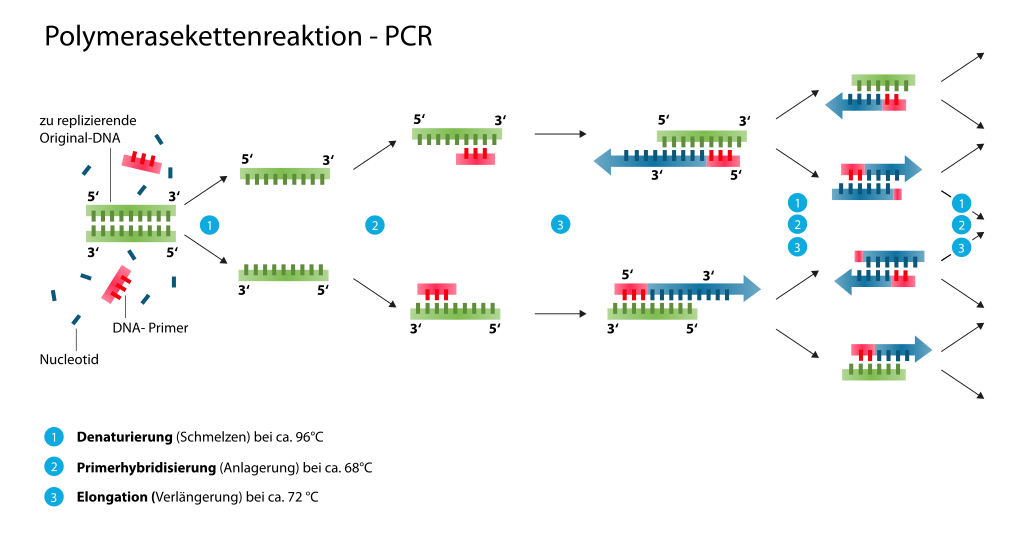
\includegraphics[width=1\textwidth]{pix/exercise1/1024px-Polymerasekettenreaktion.png}

zu amplifizierende Sequenz:\\
5‘ACCGCGGCTT AGGAAAXXXX XXXXXXCCCG GGGCGTATGC TGACGG3‘\\
\noindent\hspace*{17mm}3'-CGAA TCCTTT-5'\hspace*{23mm}3'-GGGC CCCGCA-5'

\subsection{Aufgabe 6}
Didesoxymethode nach Sanger\footnote{\url{https://de.wikipedia.org/wiki/DNA-Sequenzierung\#Didesoxymethode_nach_Sanger}}:
\begin{itemize}
	\item Didesoxynukleotide weil: wird als Stopp-Nukleotiden benutzt, an Ribose (Zucker) an Position 2' und 3' desoxidiert ist. Dadurch fehlt am 3'-Kohlenstoff-Atom die Hydroxygruppe, an der bei der Polymerisation das nächste Nukleotid angehängt wird.
	\item auch Desoxynukleotide weil: sonst funktioniert die Verlängerung nicht
	\item Ergebnis nur Didesoxynukleotide: es gibt keine Verländerung
\end{itemize}
nur Didesoxynukleotide

\newpage
\section{Übung 2}

\subsection{Aufgabe 1}
\textbf{a.)}\\
Als Crossing-over\footnote{\url{https://de.wikipedia.org/wiki/Crossing-over}} wird in der Genetik eine kreuzweise Überlagerung zweier Chromatiden mit nachfolgendem, gegenseitigem Austausch von Abschnitten bezeichnet, wie er zwischen väterlichen und mütterlichen homologen Chromosomen bei einer Meiose auftreten kann.
\\\\

\textbf{b.)} A und B sind rekombiniert zu C,D,E

\textbf{c.)} A, D,E sind rekombiniert mit B,C

\textbf{zu b.)}\hspace*{65mm}\textbf{zu c.)}\\\\
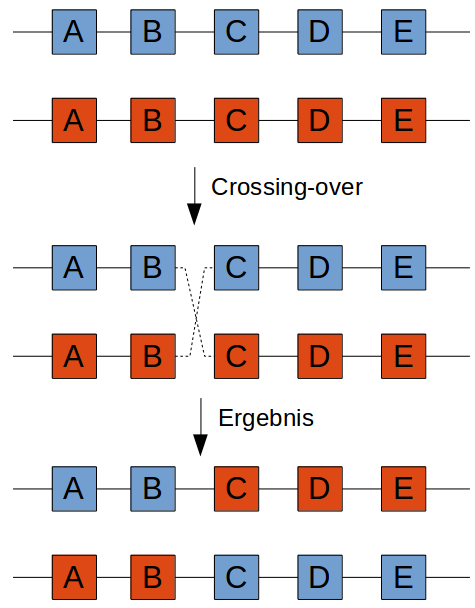
\includegraphics[width=0.5\textwidth]{pix/exercise2/crossing_over_b.png}
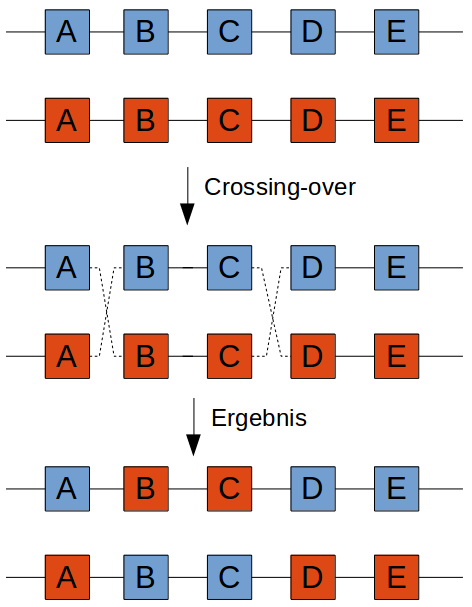
\includegraphics[width=0.5\textwidth]{pix/exercise2/crossing_over_c.png}

\subsection{Aufgabe 2}
Gen: ABO\footnote{\url{http://www.snpedia.com/index.php/ABO}}
rs8176719\footnote{\url{http://www.snpedia.com/index.php/rs8176747}}:
\begin{itemize}
	\item (-;-): likely to be of blood type O
	\item (-;G): most likely to be of blood type A or B
	\item (G;G): most likely to be of blood type A, B or AB 
\end{itemize}

rs8176747\footnote{\url{http://www.snpedia.com/index.php/rs8176747}}:
\begin{itemize}
	\item G führt zu Blutgruppe A, C zu Blutgruppe B
\end{itemize}

rs8176750\footnote{\url{http://www.snpedia.com/index.php/rs8176750}}: definiert Untergruppe von A
\begin{itemize}
	\item (-;C): A1
	\item (-;-): A2
\end{itemize}

Kombinationsmöglichkeiten:
\begin{itemize}
	\item praktisch durch Allele vorgegeben: $3 \cdot 2 \cdot 2 = 12$\footnote{\url{https://sites.google.com/site/abobloodgroup/14.aboalleles\%28oalleles\%29}}
	\item theoretisch: $5^3=125$
	\item \underline{Musterlösung:} 3 SNPs auf einem Allel $\rightarrow$ 8 Kombinationen; 2 Allele: 36 Möglichkeiten
\end{itemize}

A und B kodominant, Faktor 0 rezessiv

\subsection{Aufgabe 3}

\textbf{a.)}

\textbf{b.)}

\textbf{c.)}

\subsection{Aufgabe 4}

\textbf{a.)}\\
\underline{rezessiv:}\footnote{\url{https://de.wikipedia.org/wiki/Rezessiv}} bedeutet in der Genetik „zurücktretend“ oder auch „nicht in Erscheinung tretend“

\underline{dominant:}\footnote{\url{https://de.wikipedia.org/wiki/Dominanz_(Genetik)}} ein dominantes Allel setzt sich in der Merkmalsausprägung gegenüber einem rezessiven Allel durch

\underline{Penetranz:}\footnote{\url{https://de.wikipedia.org/wiki/Penetranz_(Genetik)}} prozentuale Wahrscheinlichkeit, mit der ein bestimmter Genotyp zur Ausbildung des zugehörigen Phänotyps führt
\\\\
\textbf{b.)}\\
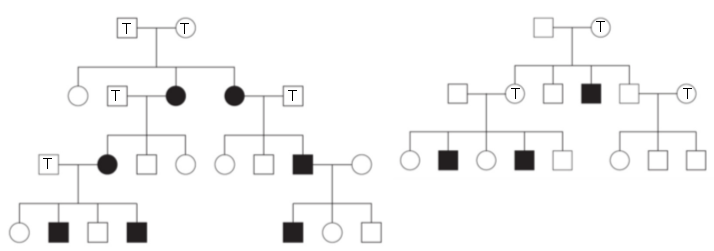
\includegraphics[width=1\textwidth]{pix/exercise2/stammbaeume1.png}
\newpage
\underline{aus Musterlösung:}\\
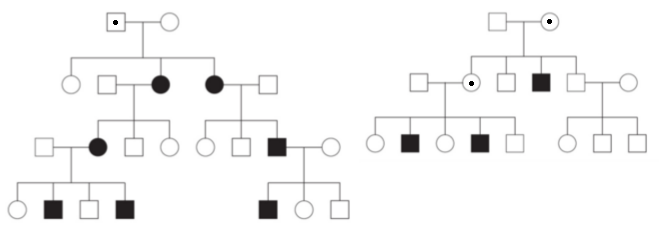
\includegraphics[width=1\textwidth]{pix/exercise2/standard_solution.png}
\\\\
\textbf{c.)}\\
\underline{links:} autosomal rezessiv, \underline{aus Musterlösung:} autosomal dominat mit reduzierter Penetranz, weil:
\begin{itemize}
	\item beide Geschlechter betroffen
	\item in jeder Generation
	\item etwa die Hälfte der Kinder betroffen
\end{itemize}

\underline{rechts:} genosomal rezessiv, auf einem X-Chromosom der Mutter\\

\newpage
\section{Übung 3}
\subsection{Aufgabe 1}
\textbf{a.)}
\begin{itemize}
	\item Sensitivität: gibt den Anteil der korrekt als positiv klassifizierten Objekte an der Gesamtheit der tatsächlich positiven Objekte an ($\mathbb{P}(P|K)$)
	\item Spezifität: gibt den Anteil der korrekt als negativ klassifizierten Objekte an der Gesamtheit der in Wirklichkeit negativen Objekte an ($\mathbb{P}(\overline{P}|\overline{K})$)
	\item Prävalenz: welcher Anteil der Menschen einer bestimmten Gruppe (Population) definierter Größe zu einem bestimmten Zeitpunkt an einer bestimmten Krankheit erkrankt ist\\
	Prävalenz=Anzahl der zum Untersuchungszeitpunkt Kranken / Anzahl der in die Untersuchung einbezogenen Individuen
\end{itemize}

\underline{Vierfeldertafel}\\
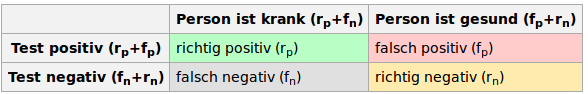
\includegraphics[width=1\textwidth]{pix/exercise3/Konfusionsmatrix.png}
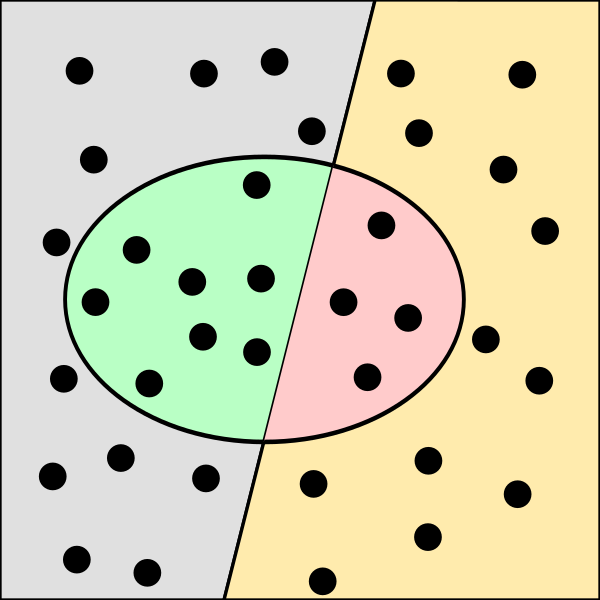
\includegraphics[width=0.5\textwidth]{pix/exercise3/Binary-classification-file.png}
\newpage
\textbf{b.)}\\
gegeben:
\begin{itemize}
	\item K=\{Patient ist krank\}
	\item P=\{Test ist positiv\}
	\item Sensitivität: $\mathbb{P}(P|K)=0,95$
	\item Spezifität: $\mathbb{P}(\overline{P}|\overline{K})=0,90$
	\item Prävalenz: $\mathbb{P}(K)=0,1$
\end{itemize}

gesucht:\\
\begin{itemize}
	\item positiv prädiktiver Wert (PPW): \\
	$\mathbb{P}(K|P) = \underbrace{\frac{\mathbb{P}(P|K) \cdot \mathbb{P}(K)}{\mathbb{P}(P)}}_{Satz\ von\ Bayes} = \underbrace{\frac{\mathbb{P}(P|K) \cdot \mathbb{P}(K)}{\underbrace{\mathbb{P}(P|\overline{K})}_{=1-\mathbb{P}(\overline{P}|\overline{K})} \cdot \mathbb{P}(\overline{K}) + \mathbb{P}(P|K) \cdot \mathbb{P}(K)}}_{totale\ Wahrscheinlichkeit}$\\
	$\mathbb{P}(K|P) = \frac{0,95 \cdot 0,1}{0,1 \cdot 0,9 + 0,95 \cdot 0,1} = $ \underline{\underline{0,513513514}}
	\item negativ prädiktiver Wert (NPW):\\
	$\mathbb{P}(\overline{K}|\overline{P})= \frac{\mathbb{P}(\overline{P}|\overline{K}) \cdot \mathbb{P}(\overline{K})}{\underbrace{\mathbb{P}(\overline{P})}_{1-\mathbb{P}(P)}} = \frac{\mathbb{P}(\overline{P}|\overline{K}) \cdot \mathbb{P}(\overline{K})}{1 - (\mathbb{P}(P|\overline{K}) \cdot \mathbb{P}(\overline{K}) + \mathbb{P}(P|K) \cdot \mathbb{P}(K))}$\\
	$\mathbb{P}(\overline{K}|\overline{P})= \frac{0,9 \cdot 0,9}{1-(0,1 \cdot 0,9 + 0,95 \cdot 0,1)} =$ \underline{\underline{0,993865031}}
\end{itemize}

\textbf{c.)}
\\
gegeben:
\begin{itemize}
	\item Sensitivität: $\mathbb{P}(P|K)=0,95$
	\item Spezifität: $\mathbb{P}(\overline{P}|\overline{K})=0,90$
	\item Prävalenz: $\mathbb{P}(K)=0,05$
\end{itemize}

gesucht:\\
\begin{itemize}
	\item positiv prädiktiver Wert (PPW)= \underline{\underline{0,$\overline{33}$}}
	\item negativ prädiktiver Wert (NPW)= \underline{\underline{0,997084548104956}}
\end{itemize}

\textbf{d.)}
siehe R-Script

\subsection{Aufgabe 2}

\subsection{Aufgabe 3}
siehe R-Script

\newpage
\section{Übung 4}
\subsection{Aufgabe 1}
siehe R-Script

\subsection{Aufgabe 2}
siehe R-Script

\subsection{Aufgabe 3}
siehe R-Script

\subsection{Aufgabe 4}
siehe R-Script

\newpage
\section{Übung 5}
\subsection{Aufgabe 1}
siehe R-Script

\subsection{Aufgabe 2}
siehe R-Script

\subsection{Aufgabe 3}

\subsection{Aufgabe 4}
siehe R-Script

\newpage
\section{Übung 6}
\subsection{Aufgabe 1}
siehe R-Script

\subsection{Aufgabe 2}

\subsection{Aufgabe 3}
siehe R-Script

\subsection{Aufgabe 4}
siehe R-Script

\newpage
\section{Übung 7}
\subsection{Aufgabe 1}

\subsection{Aufgabe 1}
siehe R-Script

\newpage
\section{Übung 8}
\subsection{Aufgabe 1}

\subsection{Aufgabe 2}
\begin{tabularx}{\textwidth}{|p{0.11\textwidth}|p{0.40\textwidth}|p{0.40\textwidth}|}
\hline
& LIFE-Adult (N=10000) & LIFE-Heart (N=7000) \\
\hline
Design & Zunächst Querschnittstudie & Kohortenstudie \\
\hline
Frage (konkret) & Identifizierung molekulargenetischer und umweltbedingter Faktoren für komplexer Erkankungen $\rightarrow$ Volkskrankheit & Identifizierung von Lebensstil- und molekulargenetischer Modifikatorebn des Atherosklerose-Risiko und verwandter Phänotypen (z.B. Lipidmetabolismus) \\
\hline
Frage (generell) & Wie gesund oder Krank ist die Bevölkerung? & Was haben die Kranken gemeinsam, sodass sich krankheiten entwickeln? \\
\hline
Vorteil & Billig, einfach durchführbar & Erfassung der Inzidenz eines Endpunktes und zeitlichen Zusammenhang zwischen Risikofaktor und Endpunkt \\
\hline
Nachteil & Ursache-Wirkung schlecht abbildbar & Teuer, seltene Endpunkte können nicht erfasst werden, selection bias\\
\hline
\end{tabularx}

\subsection{Aufgabe 3}
Sie haben in der Vorlesung den Begriff Coverage kennengelernt.\\
\begin{enumerate}
	\item Von was hängt die Coverage einer Microarrays ab?
	\begin{itemize}
		\item „Qualität meines Arrays“, wie viel Prozent des Array-SNPs sind in hinreichend hohem LD mit den Refernz-SNPs.
		\item Nimm Array-SNP und prüfe, ob dieser in der Referenz vorkommt bzw. in LD mit der Referenz-SNPs ist. Coverage ist der Anteil der in der Referenz vorkommenden SNPs
		\item Abhängig von Referenz, Ethnien, LD-Niveau, cutt-off für seltene Varianten
	\end{itemize}
	\item Was sind die üblichen Referenz-Panels und wie unterscheiden diese sich? 
international HapMap Project, 1000 Genomes Project
	\item Beschreiben Sie stichpunktartig den Workflow der Affymetrix Axiom Plattform!
\end{enumerate}

\subsection{Aufgabe 4}

\newpage
\section{Übung 9}
\subsection{Aufgabe 1}
\textbf{a.)} Was sind Batch-Effekte?\\
eine technische Quelle für Variation in den Daten durch die Verarbeitung\footnote{\url{http://www.molmine.com/magma/global_analysis/batch_effect.html}}
\\\\
\textbf{b.)} Durch was können sie entstehen, wie kann man sie vermeiden?\\
mögliche Quellen:
\begin{itemize}
	\item \textbf{Spotting:} Die Menge der Probe in den Nadeln des Roboters, der damit das Array behandelt, kann leicht variieren.
	\item \textbf{PCR Amplikation:} Proben, die durch die Polymerase-Kettenreaktion(PCR) erzeugt werden, enthalten oft nicht die gleichen Vielfachen einer Sequenz, da die Amplikation der unterschiedlichen Nukleotidstränge mit unterschiedlicher Geschwindikeit verlaufen kann.
	\item \textbf{Probenaufbereitung:} bei der Vorbereitung der Proben ist eine Vielzahl komplexer biochemischer Reaktionen, wie zum Beispiel die reverse Transkription, durchzuführen. Diese können von Labor zu Labor und innerhalb eines Experiments Unterschiede aufweisen.
	\item \textbf{RNA-Abbau:} Unterschiedliche RNA-Stränge haben aufgrund ihrer Sekundärstruktur eine unterschiedliche Halbwertszeit. Um sie zu stabilisieren, werden eine Vielzahl von Gegenmaßnahmen angewendet, die auch Nebeneffekte nach sich ziehen können.
	\item \textbf{Array-Beschichtung:} Sowohl die Effizienz der Probenfixierung auf dem Array, als auch die Intensität des Hintergrundrauschens hängt stark von der Array-Beschichtung mit der Probe ab.
\end{itemize}
Diese Probleme sollten beim Design eines Mircoarray-Experiments beachtet werden. Kann man trotz allem einen Fehler nicht verhindern, so sollten die experimentellen Bedingungen so gewählt werden, dass die biologische Fragestellung nicht beeinflusst wird. Falls zum Beispiel ein Vergleich zwischen zwei Tumorprob en durchgeführt werden soll, so ist es ratsam, beide Prob en nicht in verschiedenen Labors aufbereiten zu lassen.\footnote{\url{http://www-stud.rbi.informatik.uni-frankfurt.de/~linhi/SeminarSS04/Ausarbeitungen/03ausarbeitung_evgenji_yusuf.pdf}}
\\\\
\textbf{c.)} Erinnern Sie sich an Aufgabe 4 von Blatt 6. Statt verschiedener Populationen nehmen wir nun an, dass der SNP auf verschiedenen Platten gemessen wurde. Führen Sie einen Chi-Quadrat-Test durch, ob sich die Allelhäufigkeiten zwischen den Platten signifikant unterscheidet!\\\\
Ergebnisse siehe R-Skript

\subsection{Aufgabe 2}
siehe R-Script (prüfungsrelevant: Plots und Inhalte bewerten)

\subsection{Aufgabe 3}
\textbf{a.)}\\
siehe vorherige Aufgabe, Outlier außerhalb von Clustern\\\\
\textbf{b.)}\\
Callrate ausrechnen, wenn Callrate $<$ 97\% $\rightarrow$ Missings entfernen\\\\
\textbf{c.)}\\
Imputation:
\begin{enumerate}
	\item \underline{Referenzabgleich:} Welche Array-SNPs sind in der Referenz und sind sie gleich codiert? (ID, Chromosom, Position, Strang, Allel A, Allel B)
	\item Phasierung: Schätzung der Haplotypen
\end{enumerate}

\newpage
\section{Übung 10}
\subsection{Aufgabe 1}
siehe R-Skript (Prüfungsrelevant: QQ-Plot bewerten (Grenze beachten), Manhatten-Plot (Signifikanzgrenzen beachten))\\
signifikante Assoziation zwischen betrachteten SNP und phenotypischen Merkmal\\
so viele grüne übereinander da in einem Block (ohne Korrektur durch LD)

\subsection{Aufgabe 2}
\textbf{a.)}
\begin{itemize}
	\item Haplotyp\footnote{\url{https://de.wikipedia.org/wiki/Haplotyp}}: Variante einer Nukleotidsequenz auf ein und demselben Chromosom im Genom eines Lebewesens
	\item Haploblock: Haplotypen verschiedener Individuen als Block geschrieben sind ein Haploblock
	\item Rekombinations-Hotspot\footnote{\url{https://en.wikipedia.org/wiki/Recombination_hotspot}}: Bereich im Genom der eine erhöhte Rekombinationsrate im Vergleich zur neutralen Erwartung aufweist
\end{itemize}

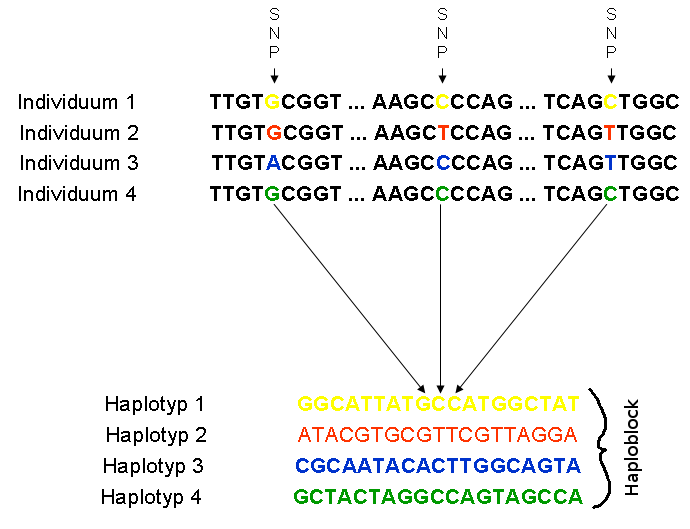
\includegraphics[width=0.5\textwidth]{pix/exercise10/Haplotyp.PNG}\\
Haplotypen aus SNPs von Chromosomenabschnitten des gleichen Chromosoms von vier haploiden Individuen
\\\\
\textbf{b.)}\\
862 weitere SNPs auf Gen ABO\footnote{Vorgehen siehe \url{https://www.ncbi.nlm.nih.gov/guide/howto/view-all-snps/}}

Aus snpedia: 36

\textbf{c.)}\\
Durch die drei bekannten SNPs sind die relevanten Haploblöcke vollständig beschrieben\\
\textbf{d.)}\\
wenige SNPs reichen aus, um den Genotyp der restlichen SNPs im Block zu bestimmen

\subsection{Aufgabe 3}
\textbf{a.)}\\
Mischen von fixed- und random-Effects\\
\textbf{b.)}\\
y$_{ijk}=\mu+\beta_{j}+b_{j}+\epsilon_{ijk}$\\
Proband: i=1-6\\
Ergometer: j=1-3
Wiederholung: k=1-3\\
$\beta_j$: Effekt des Ergometers j (fixer Effekt)\\
$b_{i}$: Effekt des Probanden i (zufälliger Effekt, Variation innerhalb der Probanden)\\
jeder Proband hat seine eigenen Intercept, aber alle haben die gleiche Steigung\\
Beispiel oben: Random Intercept Modell == fixed effect meta analyse, denn Studien haben eigenen Intercept\\

\textbf{c.)}

\textbf{d.)}

\end{document}